\subsection{Abzubildender Workflow}\label{l:workflow}

Hauptaufgabe der Anwendung ist es, den Workflow von der Definition bis zur Übernahmen der fertigen Texte in das Produkt zu übernehmen und dabei nicht nur Funktionen zur \emph{Definieren} und \emph{Speichern} und \emph{Exportieren} zu bieten, sondern auch die \emph{Kommunikation über die Texte} zu integrieren. Für die Umsetzung des Workflows in einer Anwendung müssen zunächst alle Ausprägungen der speziellen Abläufe beschrieben werden. In Abschnitt \ref{l:besondererolle} wurde bereits beschrieben, wie umfangreich die Anzahl der Personen ist, die Einfluss auf die Texte eines Produktes haben. Die Rollenverteilung ist dabei von Projekt zu Projekt unterschiedlich, mit den in Kapitel \ref{l:personas} vorgestellten Personas würde eine Übersicht über die typische Rollenverteilung geschaffen. Betrachtet man die von Projektmitarbeitern durchgeführten Operationen in Zusammenhang mit Text lassen sich diese in sechs eigenständige Operationen unterteilen:

\begin{enumerate}
\item Durch \textbf{Definieren eines Textbausteines} werden dessen \emph{Attribute} bestimmt. Dadurch wird festgelegt, wie der benötigte Text beschaffen sein muss. Die Aussage \citequotes{Wir brauchen an dieser Stelle eine Überschrift} ist ein Beispiel für diese Operation. Sie legt fest, wie der Textbausteine gestaltet werden muss, um die ihm zugedachte Aufgabe zu erfüllen. Neben der Angabe zur Platzierung auf dem Medium durch \typoquotes{an dieser Stelle} wird implizit durch \typoquotes{eine Überschrift} eine Angabe zur inhaltlichen und visuellen Gestaltung getroffen; Überschriften sollen kurz und knapp sein und ihre visuelle Gestaltung wird durch den Styleguide des Projekts festgelegt.
\item Das \textbf{Schreiben eines Textes} erzeugt den Inhalt eines Textbausteins in einer Sprache. Bei diesem Vorgang wird der Text entsprechend der Vorgabe aus der Beschreibung als Original erstellt oder aus Quellen außerhalb des Projekts kopiert und eingefügt.
\item In der \textbf{Korrektur} wird der Text inhaltlich und grammatikalisch überprüft und entsprechend angepasst. Der Korrektor muss dabei für eine grammatikalische Überprüfung des Textes kein Fachwissen bezogen auf das Projekt haben. Ist diese Fachwissen vorhanden, kann eine inhaltliche Korrektur vorgenommen werden.
\item In der \textbf{Qualitätskontrolle} wird der Text dahingehend überprüft, ob er den Anforderungen gemäß der Beschreibung und inhaltlichen Vorgaben, auch hinsichtlich des gesamten Projekts entspricht.
\item Durch die \textbf{Freigabe} wird der Text abgenommen und kann nun in das Endprodukt übernommen werden. Die Freigabe unterscheidet sich von der Qualitätskontrolle durch ihren authorativen Charakter. Qualitätskontrolle können prinzipiell von allen Mitarbeitern durchgeführt werden. Freigaben werden nur von Mitarbeitern mit Management-Berechtigungen erteilt.
\item Durch die \textbf{Veröffentlichung} wird der Text in das Endprodukt eingebracht.
\end{enumerate}

\begin{samepage}
Verallgemeinert man diesen Ablauf, erkennt man, dass sich der Einfluss in drei grundlegenden Eigenschaften der Texte unterteilen lässt:

\begin{enumerate}\itemsep -5pt
\item den \textbf{Inhalt} des Textes,
\item die \textbf{Attribute} wie z.B. \typoquotes{maximale Textlänge} oder \typoquotes{Position im Medium}
\item und den \textbf{Status} wie z.B. \typoquotes{neu} und \typoquotes{freigegeben}.
\end{enumerate}
\end{samepage}

Das Gewicht des Einfluss der Mitarbeiter ist je nach Rolle unterschiedlich, Tabelle \ref{table:texteinfluss} · S.\pageref{table:texteinfluss} zeigt dies in einer Übersicht.

\begin{table}
\begin{center}
\begin{tabular}{@{}r c c c}
\textbf{Persona} & \textbf{Inhalt} & \textbf{Attribute} & \textbf{Status}\\[1ex]
\textbf{Agentur} & & & \\
\hline\\[-1.5ex]
\emph{Eva}, Konzept & \HarveyQuarter & \HarveyFull & \HarveyEmpty \\
\emph{Lotte}, Art-Direktion & \HarveyEmpty & \HarveyThreeQuarters & \HarveyEmpty \\
\emph{Jan}, Produktion & \HarveyEmpty & \HarveyQuarter & \HarveyEmpty \\
\emph{Arthur}, Projektleitung & \HarveyEmpty & \HarveyEmpty & \HarveyQuarter \\[1ex]
\textbf{Extern} & & & \\
\hline\\[-1.5ex]
\emph{Torsten}, Text & \HarveyHalf & \HarveyEmpty & \HarveyEmpty \\
\emph{Jorinde}, Übersetzung & \HarveyQuarter & \HarveyEmpty & \HarveyEmpty \\[1ex]
\textbf{Kunde} & & & \\
\hline\\[-1.5ex]
\emph{Markus} & \HarveyHalf & \HarveyQuarter & \HarveyFull
\end{tabular}
\caption{Stärke des Einfluss, die Mitarbeiter in einem Projekt haben}
\label{table:texteinfluss}
\end{center}
\end{table}

\bigskip

Nachfolgend sind die Text-Eigenschaften näher beschrieben.

\subsubsection{Inhalt}

Personen die Einfluss auf den \emph{Inhalt} haben, sind vor allem diejenigen die die Texte für das Produkt liefern. Neben den Mitarbeitern auf Kundenseite, Ausgangsmaterialien und Fachinformationen zur Verfügung stellen sind die Texter und Übersetzer, die diese Informationen aufbereitet. Texte müssen aber auch die die spezifischen Gegebenheiten des Mediums angepasst werden, hierzu liefern Experten Rahmenbedingungen aber auch inhaltliche Anpassungen. Ein Beispiel hierfür ist die Suchmaschinenoptimierung (SEO) von Texten. Hierbei werden Texte auf das Vorhandensein von bestimmte Formulierungen und Stichwörter optimiert aber auch Vorgaben über die Länge und Aufbau von Texten gemacht. 

Mit Inhalt ist der eigentliche Text gemeint, der auch im Produkt erscheint. Für Inhalte gibt es immer eine Original-Version für die im späteren Projektverlauf Übersetzungen in eine oder mehrere Sprachen angelegt werden können. Die Übersetzung basiert dabei auf der Original-Version, oder je nach Übersetzer auch auf einer anderen Übersetzung.

Vorgaben für Inhalte werden in Form von Richtlinien formuliert. Diese Richlinen dienen dem Texter als Orientierungshilfe, wie er die Texte zu formulieren hat. Richtlinien werden von verschiedenen Mitarbeitern formuliert: 
\begin{itemize}\itemsep -5pt
\item Vom Konzept werden grundlegende Vorgaben geschaffen, wie z.B. Annahmen über die Zielgruppe und den Zweck des Produktes.
\item Der Kunde hat Vorstellungen oder sogar Vorgaben, wie der Sprach-Stil der Texte sein soll, aus seinen Fachabteilungen und von Beratern oder Anwälten werden weitere Vorgaben über erwünschte oder zu vermeidende Aussagen erstellt.
\end{itemize}
Es existieren aber auch implizite Vorgaben, die sich aus der Art des Mediums ergeben: Lange Texte sind für Fernsehspots ungeeignet, Informationsbröschüren haben Raum für ausführliche Erläuterungen.

Nicht selten werden weitere externe Experten zu Projekten hinzugezogen, die Texte auf bestimmte Aspekte hin anpassen. Besonders bei Internetseiten werden SEO-Konzepte erstellt, auf deren Basis die Texte von einzelnen Seiten und Abschnitten so angepasst werden, dass diese bestimmte Schlüsselwörter und Formulierungen enthalten, um von den Algorithmen der Suchmaschinenbetreiber bessere Positionierungen in Suchergebnissen zu erreichen.

\subsubsection{Attribute} 

Attribute legen die Rahmenbedingungen von Text fest, diese werden vor allem in der Gestaltung des Produktes durch Designer, als auch in der Umsetzung durch produktbedingte Einschränkungen, z.B. Platzverhältnisse oder systembedingte Beschränkungen, bestimmt. Attribute sind in irgendeiner Form quantifizierbare Angaben zu Textbausteinen. Sie dienen zum einen dazu, den Textbaustein zu identifizieren und seine Rolle im Produkt festzulegen und zum anderen werden damit Vorgaben zur Beschaffenheit des Textes festgelegt. Die Attribute lassen sich in vier Bereiche unterteilen:

\paragraph{Identifier} Dies sind eindeutige Bezeichner für Textbausteine, diese dienen dazu, Referenzen zwischen den Textbausteinen im System und im Produkt herzustellen, z.B. um automatische Aktualisierungen zu ermöglichen. Identifier werden auch benötigt, damit Kommentare, Zusatzinformationen usw. diesen eindeutig zugordnet werden können.

\paragraph{Klasse} generell lassen sich die Texte in jedem Produkt in wenige, deutlich unterscheidbare Klassen unterteilen. Aus Gründen der Usability versucht man bei der Gestaltung von Medien ein einheitliches Gestaltungsbild zu erreichen, dazu gehört auch, dass Texte, die die gleiche Funktion haben, auch gleich gestaltet werden. In den meisten Fällen gibt es eine Unterscheidung zwischen Fließtext und Überschriften, die es auf mehreren Hierarchieebenen gibt. Bei interaktiven Produkten finden sich dann häufig Texte für Navigations-Elemente wie Buttons und Links oder für die Verwendung in Formularen. Bei der Klassifizierung von Texten werden die Schriftart, Schriftgröße, Schreibweise  (z.B. nur GROSSBUCHSTABEN) und weitere Angaben zu Formatierung (z.B. Abstände zum nächsten Textbaustein) bestimmt, die für alle Texte dieser Klasse verwendet werden. Zusätzlich werden üblichweise auch noch weitere Regeln für die Verwendung der Klassen festgelegt, z.B. dass auf eine Headline immer vor einem Fließtext stehen muss. Teil der Klassifizierung können auch Angaben zur Zeichenlänge enthalten, da dies aber nicht immer zwingend der Fall ist und es auch Textlängenbeschränkungen ohne Bezug zur Klasse eines Textes geben kann (z.B. bei Forumularen) werden diese separat betrachtet.

\paragraph{Textlänge} In vielen Fällen ist es aus gestalterischer, inhaltlicher oder technisches Sicht gewünscht, dass die Textlänge eines Textbausteines in einem gewissen Rahmen liegt. Üblich sind Vorgaben zur minimalen, maximalen und gewünschten Anzahl von Zeichen, Wörtern, Sätzen, Zeilen und Absätzen

\paragraph{Position} Zu jedem Textbaustein wird festgelegt, wo dieser im Produkt erscheint. Diese Information ist besonders für die Produktion wichtig, aber auch schon vorher wird diese Information immer wieder benötigt, z.B. um vor Fertigstellung des Produktes eine Vorschau oder einen Dummy einzelner Bestandteile des Produktes anzufertigen. Positionsangaben bestehen meistens aus zwei Komponenten. Zum einen wird eine hierarchische Position definiert, z.B. auf \citequotes{im zweiten Kapitel}, oder \citequotes{unter der Überschrift auf der Seite \typoquotes{Über uns}.} Zum anderen kann es exakte Postionsangaben und Größenangaben geben. Diese haben zwar keinen direkten Einfluss auf den Text, können aber für Produkte mit festen Gestaltungsrahmen und den Informationen zur Textklasse wichtige Hinweise darüber liefern, wie lang der Text maximal sein darf, ohne das Layout \typoquotes{zu sprengen}.

\subsubsection{Status}\label{l:konzept-workflow-status}

Den Status von Texten, also ob ein Text dem nächsten Mitarbeiter im Workflow zugewiesen werden soll kann von bestimmten Mitarbeitern abhängen. Es ist üblich, dass Texte erst dann dem Kunden zur Abnahme vorgelegt werden, wenn sie als Gesamtes vorliegen. Auch externe Dienstleister bekommen aus Kostengründen meisten alle Text im Paket, damit eine zügige Abarbeitung des Auftrages gewährleistet wird. Praktisch ist der Status eines Textes dem aktuellen Bearbeiter gleich zu setzen. Eine Änderung des Status bedeutet, dass der aktuelle Bearbeiter seine Aufgabe abgeschlossen hat und der nächste Bearbeiter mit seiner Aufgabe weitermachen kann. Es kann auch eine Statusänderung in umgekehrter Richtung geben, wenn der die Vorbedingungen für den nächsten Mitarbeiter nicht erfüllt sind, oder bei einer Kontrolle ein Problem festgestellt wird. Je nach Mitarbeiter unterscheidet sich, zu welchen Zeitpunkt und zu welchen Status er Feedback gibt. Abbildung~\ref{chart:workflowmitfeedback} · S.\pageref{chart:workflowmitfeedback} gibt einen Überblick über die Entscheidungsprozesse im Verlauf eines Projekts und wer auf diese Einfluss nimmt. Tabelle \ref{table:workflowmitfeedback} · S.\pageref{table:workflowmitfeedback} listet den Einfluss tabellarische und enthält zusätzlich Informationen, wie stark der jeweils ausgeübte Einfluss in der Regel ist.

\begin{figure}[htb]
\begin{center}
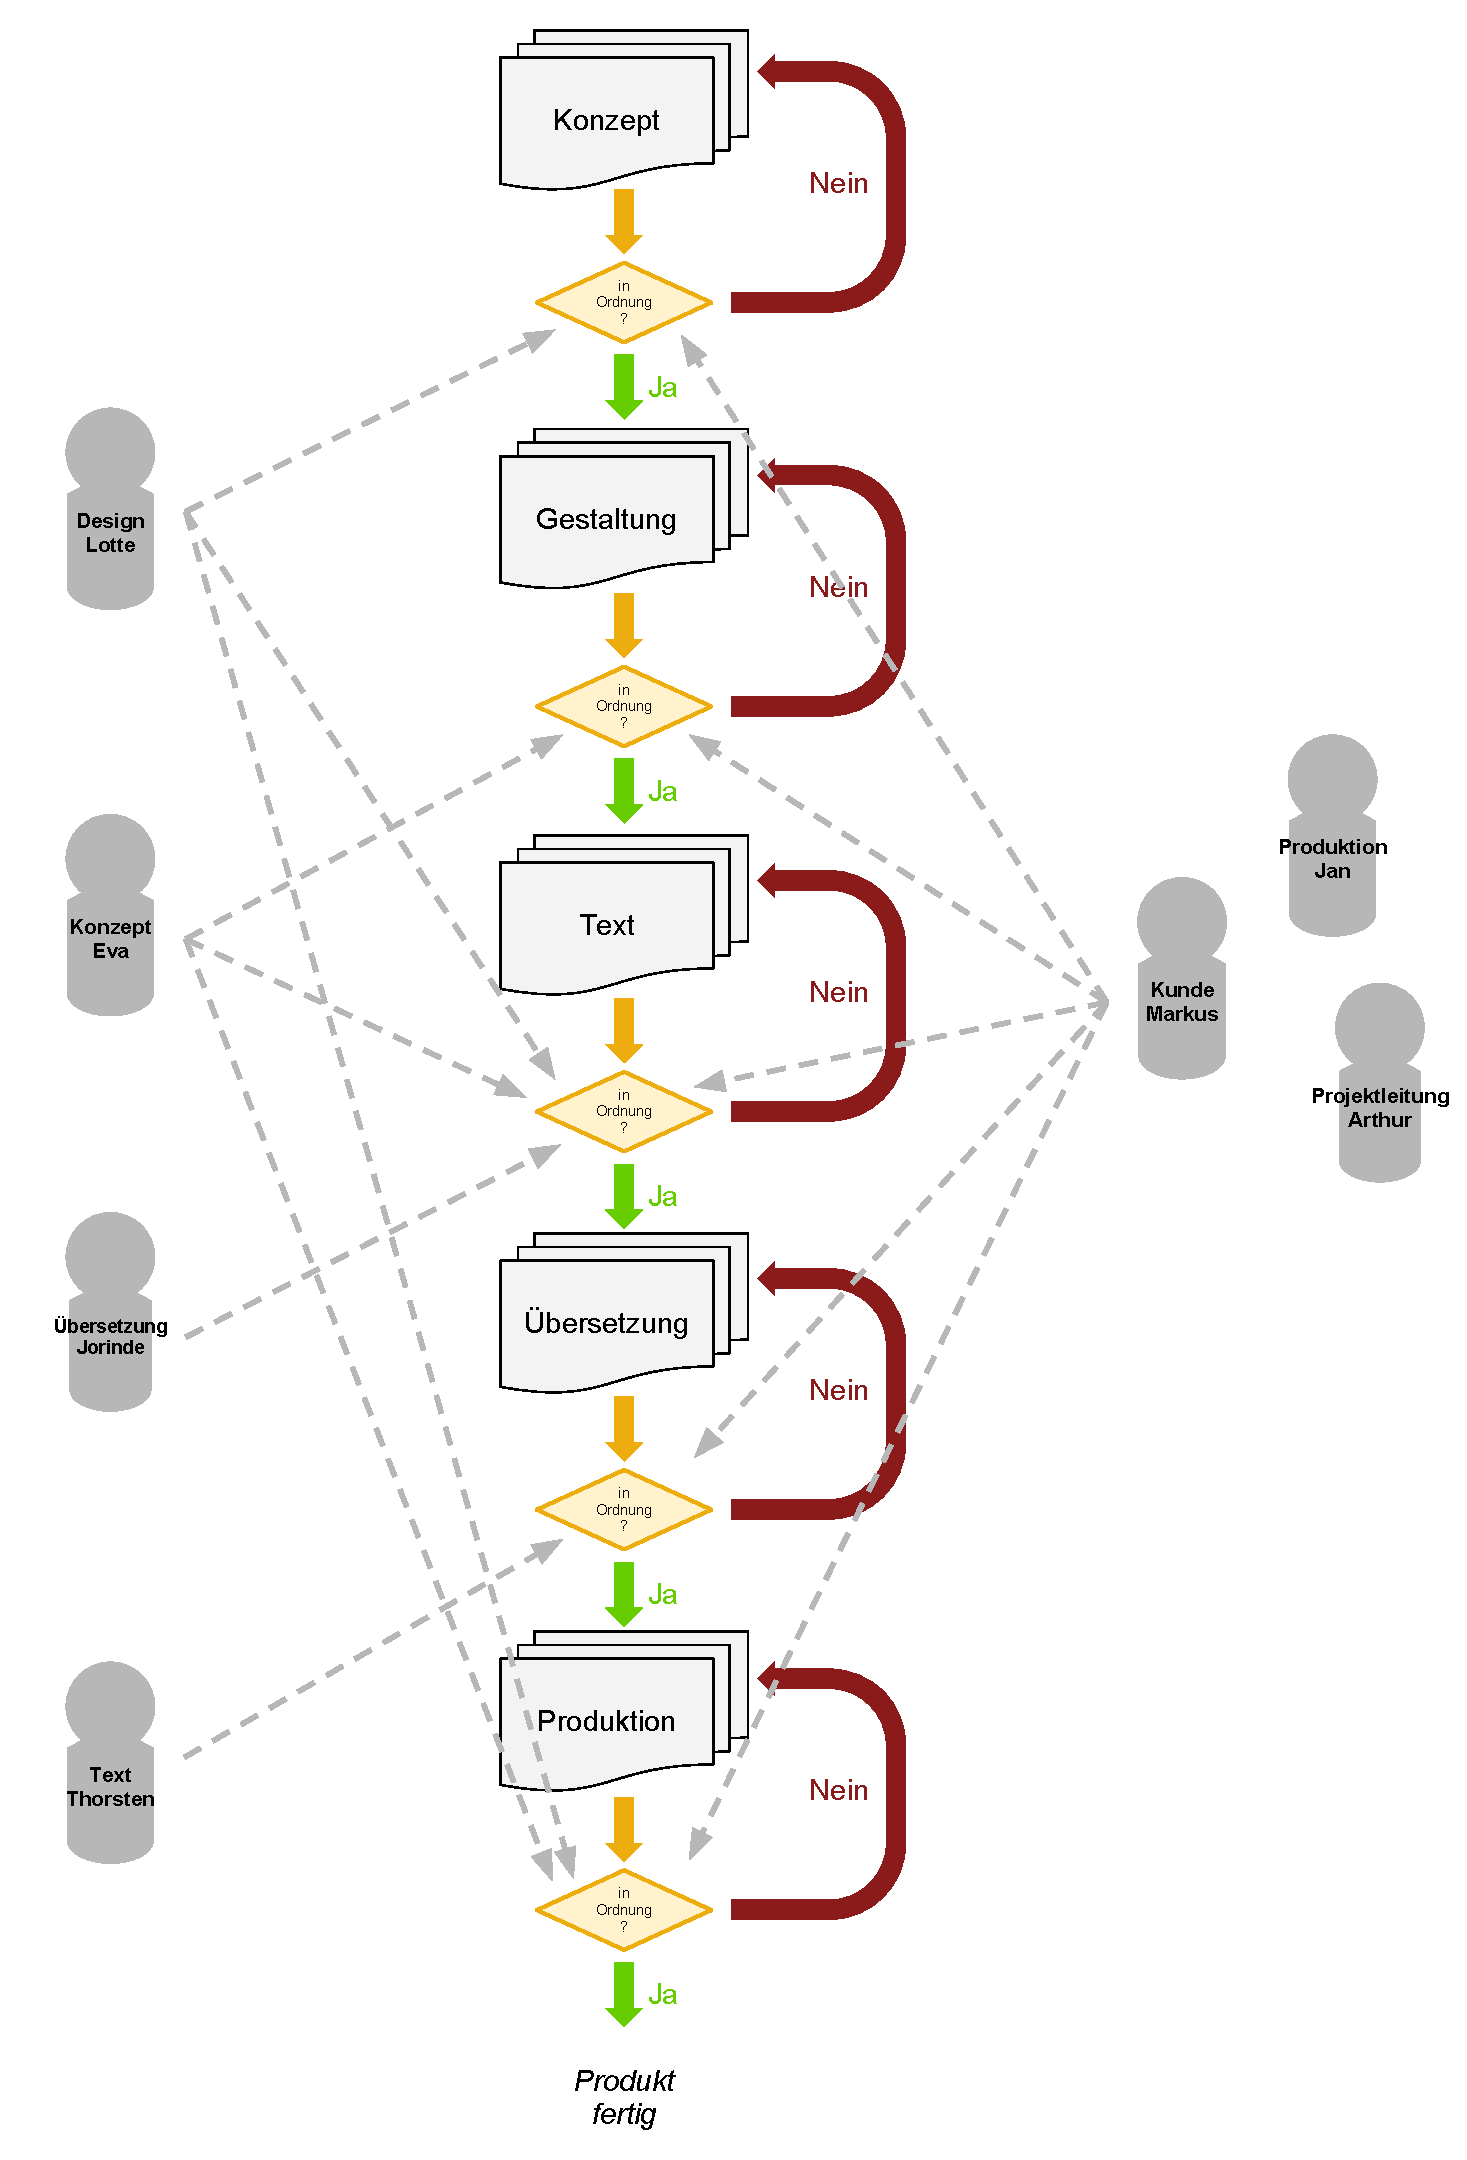
\includegraphics[width=0.6\textwidth]{media/WorkflowmitFeedback.pdf}
\end{center}
\caption{Einfluss auf den Status eines Textbausteines}
\label{chart:workflowmitfeedback}
\end{figure}

\begin{table}
\begin{center}
\begin{tabular}{@{}l c c c c c c c}
& \textbf{Eva} & \textbf{Lotte} & \textbf{Torsten} &  \textbf{Jorinde} & \textbf{Jan} & \textbf{Arthur} & \textbf{Markus}\\
{\small Einfluss auf} & {\small Konz.} & {\small Des.} & {\small Texter} & {\small Übersetz.} & {\small Prod.} & {\small Projektl.} & {\small Kunde}\\
\hline\\[-1.5ex]
Konzept & \HarveyFull & \HarveyQuarter & \HarveyEmpty & \HarveyEmpty & \HarveyQuarter & \HarveyHalf & \HarveyThreeQuarters \\
Design & \HarveyQuarter & \HarveyFull & \HarveyEmpty & \HarveyEmpty & \HarveyQuarter & \HarveyQuarter & \HarveyThreeQuarters \\
Text & \HarveyHalf & \HarveyQuarter & \HarveyFull & \HarveyQuarter & \HarveyQuarter & \HarveyQuarter & \HarveyHalf \\
Übersetzung & \HarveyEmpty & \HarveyEmpty & \HarveyHalf & \HarveyFull & \HarveyQuarter & \HarveyQuarter & \HarveyHalf \\
Produktion & \HarveyHalf & \HarveyHalf & \HarveyEmpty & \HarveyEmpty & \HarveyFull & \HarveyHalf & \HarveyFull \\
\end{tabular}
\caption{Einfluss mit Gewichtung auf den Status eines Textbausteines}
\label{table:workflowmitfeedback}
\end{center}
\end{table}

\paragraph{Ereignisse} Da sich die Texte des Produktes aus vielen einzelnen Bausteinen zusammensetzen, werden auch die Eigenschaften jeweils einzelnen gesetzt. Aus Sicht des Projektverlaufes ergeben sich aus der Gesamtheit alle Zustände bestimmte Ereignisse, die sich auf die Änderung der Stati der Texte zurückführen lassen. Immer dann, wenn alle Texte eines Produktes einen gewissen Status erreichen, werden bestimmte Ereignisse ausgelöst. Ein Beispiel: erst wenn alle Texte durch den Kunden abgenommen wurden, werden diese an die Übersetzung übergeben. Dies stellt sicher, dass die Übersetzung nur die Texte übersetzt, die auch benötigt werden und somit keine unnötigen Kosten verursacht.
